\chapter{Verification}
\label{ch:verification}
This chapter presents a validation of the design proposed in chapter~\ref{ch:architecture}.
Section~\ref{sec:test-configuration}
presents the configuration used to perform the
validation tests.
Section~\ref{sec:external-review} presents one of the most important
aspect of the validation process,
the peer review
which was more than relevant to properly assess the status of this
work, and to identify promising lines of future work,
as mentioned in chapter~\ref{ch:conclusions}.
% Finally,
% section~\ref{sec:results-comparisons}
% presents additional results and comparisons with other work.

\section{Test Configuration}
\label{sec:test-configuration}
For testing purposes two models were generated,
these models cover the full spectrum of code that can be generated by
this work.
Both models cover a basic component,
and more complicated structures as enumerated in table~\ref{tb:stereotypes}.

At the time when implementation was begun,
the setup chosen was:
\begin{itemize}
\item\textbf{Operating System}: A virtual machine with Red Hat Enterprise Linux 4.4 (interchangeable with Scientific Linux 4.4).
\item\textbf{ACS}: ACS version 8.0.0 Back port Red Hat 4.4.
\item\textbf{OAW}: Version 4.1.3 with the itemis distribution.
\item\textbf{Modeling Tool}: Magic Draw 16.5
\end{itemize}

The models used are specified in figures~%
\ref{fg:MARSclassDiagram},~%
\ref{fg:ExtendedMARSclassDiagram} and~%
\ref{fg:BACIClassDiagram}.
The MARS model~\ref{fg:MARSclassDiagram} makes full usage of support of enumerated types
and \texttt{<<IDLStructs>>}.
The BACI Example is intended to test the generation of a characteristic component
including \lstinline[language=IDL]!readWrite! and \lstinline[language=IDL]!readOnly! characteristics.

\begin{figure}
  \begin{center}
  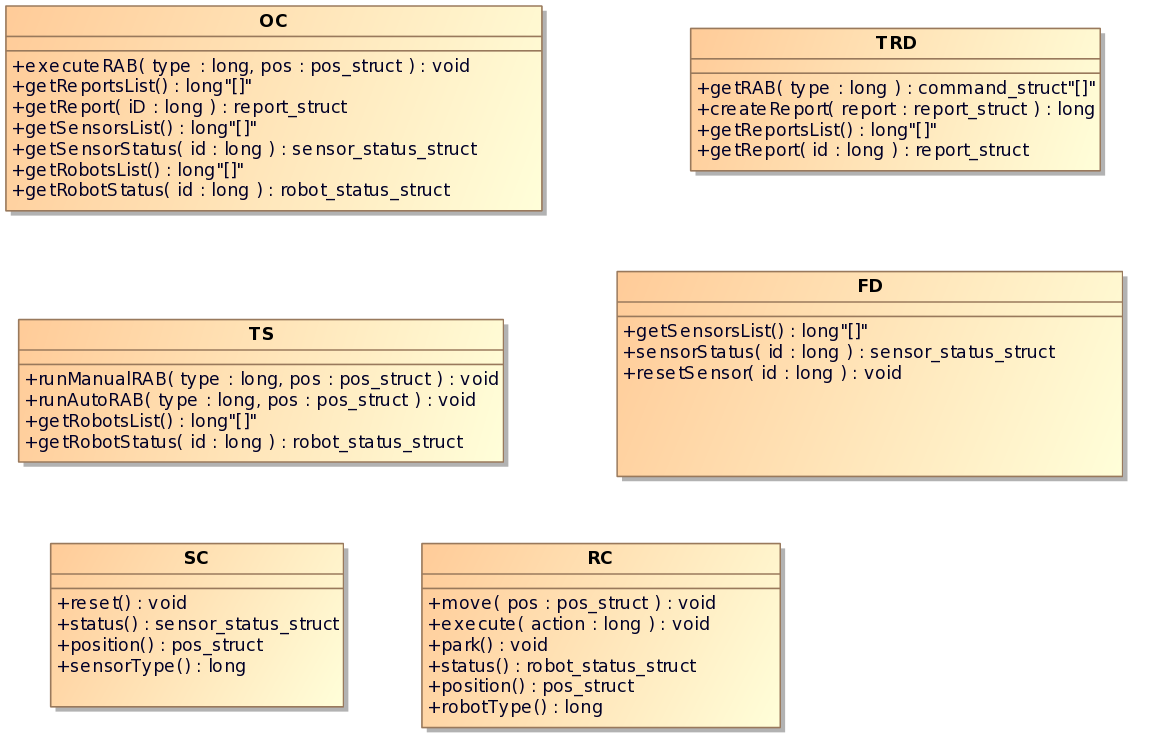
\includegraphics[width=\textwidth]{images/MARS-classdiagram.png}
% Fixme: Has grid lines in the background, text is too small to read
  \end{center}
  \caption{MARS Example Class Diagram}
  \label{fg:MARSclassDiagram}
\end{figure}


\begin{figure}
  \begin{center}
  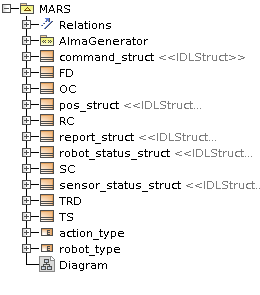
\includegraphics[width=0.65\textwidth]{images/MARS-classdiagram-full.png}
% Fixme: Completely unreadable, way too small
  \end{center}
  \caption{Extended MARS Example Class Diagram}
  \label{fg:ExtendedMARSclassDiagram}
\end{figure}

\begin{figure}
  \begin{center}
  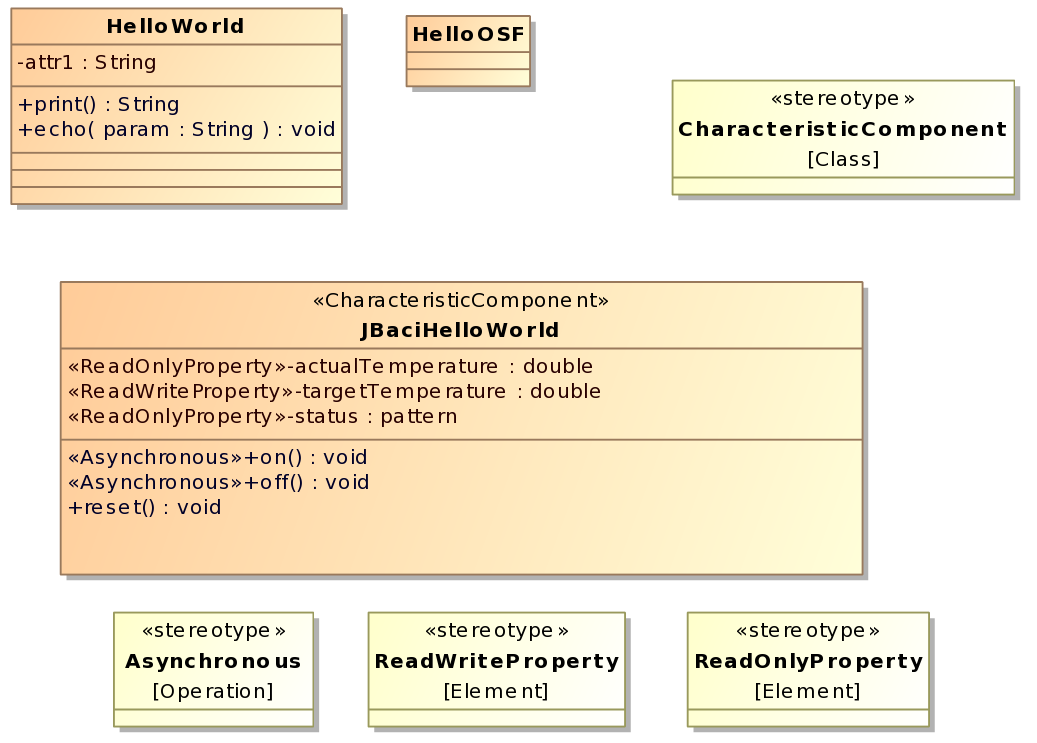
\includegraphics[width=\textwidth]{images/example-classdiagram.png}
  \end{center}
  \caption{BACI Example Class Diagram}
% Fixme: Completely unreadable, way too small
  \label{fg:BACIClassDiagram}
\end{figure}

After executing the ACS code generator as described by the workflow in
section~\ref{sec:generation-workflow},
the output files were tested initially by compiling and installing
the new software module.
Compilation is achieved using the generated \lstinline[language=sh]!Makefile!.
A strict requisite is that the generated code must
compile correctly and it should be possible to instantiate all classes.
This is manually checked during the verification process,
a test suite should be generated to automate this process.

\section{External and Peer Review}
\label{sec:external-review}
This work was followed closely by Gianluca Chiozzi,
Head of Software Instrumentation at ESO,
who had the opportunity to test preliminary versions of
the ACS code generator.
His comments and suggestions are gratefully acknowledged.
He presented a poster~\cite{chiozzi09:_acs_status} at
ICALEPCS 2009, where this generator is mentioned as
a future feature for ACS.

This work was also presented in the Advanced Track of
the 6th ACS Workshop,
which took place at UTFSM, on November $13^{th}-19^{th}$ 2009.
Positive feedback was received during
the presentations, including requests for new features which
should be addressed as future work (see section~\ref{sec:future-work}).

The MARS model (figure~\ref{fg:MARSclassDiagram}) was originally
designed for the
basic tutorial track of the 6th ACS Workshop,
but it evolved into a validation
suite for this project.
A portion of the generated code, specifically the IDL files,
was used during the basic track and a software implementation
of these IDL files
was implemented using the ACS framework.

%\section{Results and Comparisons}
%\label{sec:results-comparisons}
% As the title says results and comparison.
% Good comparison are Control Code generator
% ACS generator and state machine Generator.



%%% Local Variables:
%%% mode: latex
%%% TeX-master: "../thesis"
%%% End:
